% !TeX program = xelatex
% Closed-loop verification of Goldbach-related claims
\documentclass[11pt,a4paper]{ctexart}

\usepackage[margin=2.54cm]{geometry}
\usepackage{amsmath,amssymb,amsthm}
\usepackage{graphicx}
\usepackage{booktabs}
\usepackage{longtable}
\usepackage{array}
\usepackage{tabularx}
\usepackage{multirow}
\usepackage{enumitem}
\usepackage{caption}
\usepackage{xcolor}
\usepackage{url}
\usepackage[hidelinks]{hyperref}
\usepackage{microtype}

\setlength{\emergencystretch}{3em}
\sloppy
\raggedbottom

\captionsetup{font=small,labelfont=bf,skip=6pt}
\setlist[itemize]{leftmargin=2em,itemsep=0.25em,topsep=0.35em}
\setlist[enumerate]{leftmargin=2.2em,itemsep=0.25em,topsep=0.35em}

\theoremstyle{plain}
\newtheorem{theorem}{定理}[section]
\newtheorem{lemma}[theorem]{引理}
\newtheorem{proposition}[theorem]{命题}
\newtheorem{corollary}[theorem]{推论}
\theoremstyle{definition}
\newtheorem{definition}[theorem]{定义}
\newtheorem{remark}[theorem]{注}
\newtheorem{example}[theorem]{例}

\newcommand{\BG}{\mathrm{BG}}
\newcommand{\Chen}{\mathrm{Chen}}
\newcommand{\LL}{\mathrm{LL}}
\newcommand{\WU}{\mathrm{Wu}}
\newcommand{\Even}{\operatorname{Even}}
\newcommand{\Prime}{\operatorname{prime}}
\newcommand{\PaperTheorem}{\mathrm{PaperTheorem}}
\newcommand{\g}{\mathrm{g}}
\newcommand{\N}{\mathbb{N}}
\newcommand{\R}{\mathbb{R}}
\newcommand{\Aone}{\textsf{A1}}
\newcommand{\Atwo}{\textsf{A2}}
\newcommand{\Bclass}{\textsf{B}}
\newcommand{\Cclass}{\textsf{C}}
\newcommand{\Dclass}{\textsf{D}}

\title{\bfseries 哥德巴赫猜想相关声明的闭环核验：\\[2pt]
文本审计、机器形式化与独立闭包重建}
\author{宋敏、宋瑷成、宋奥菲、范钧睿、胡安、涂源}
\date{2026年11月17日\\[2pt]
\small 预印本 v1}

\setCJKmonofont{SimHei}

\hypersetup{
  pdftitle={哥德巴赫猜想相关声明的闭环核验：文本审计、机器形式化与独立闭包重建},
  pdfauthor={宋敏, 宋瑷成, 宋奥菲, 范钧睿, 胡安, 涂源},
  pdfkeywords={Goldbach conjecture, Lean 4, formal verification, reproducibility, evidence hierarchy}
}

\begin{document}
\maketitle

\begin{abstract}
\noindent
二元哥德巴赫猜想至今开放，但围绕它的弱型定理、初等证明与形式化工程常被混同。本文提出并执行一个四阶段闭环核验框架：声明分解与版本钉扎、逐行文本审计、可复算数值检查、Lean~4 形式化与公理审计，以及在源码清单约束下的独立闭包重建；并以 A1/A2/B/C/D 五类证据标签区分“内核定理”“产物通过”“文本事实”“有限计算”与“判断”。三个相互关联的案例给出不同结果。第一，对 arXiv:2611.09007v1，按作者自定义的 $\mathcal O$（比值趋于非零常数），其定理~1.1 的陈述已蕴含 $1+1$；证明开头把当前情形 $G(2n)$ 列入假设，构成循环；它还把 $G(2n-2)>0$ 当作输入，在字面定义下已预设结论的正性，在标准读法下则缺乏依据；式~(1)(2) 在 $3\le x\le 6000$ 上各差 $1$、方向相反。字面读法与标准 $\mathcal O$ 读法均不能支撑其证明主张。第二，8 条 Lean~4 定理表明 $1+1$ 蕴含 Chen $1+2$、Li--Liu $1+1.9$ 与 Wu $1+1.8938$，三端点的表示谓词严格更宽；但这不是独立性证明，也不构成反推。第三，对 Wu 端点的 3,764 个导入闭包模块完成本地独立重编：0 真实失败，30,215,769 字节/621,451 物理行的源哈希与清单一致，6 条端点声明恰好依赖标准三公理，端点模块 \texttt{leanchecker} 重放返回 0。该重建是产物级、非 clean-room、只覆盖导入闭包，不验证论文散文。结论：哥德巴赫猜想仍开放；闭环核验的价值不在于再喊一次“已证明”，而在于把证明主张、形式化产物、有限证据与残余不确定性分开，使否定性结论同样可审计。

\vspace{0.6em}
\noindent\textbf{关键词：}哥德巴赫猜想；形式化验证；Lean~4；可复现性；证据分级；数学审计

\vspace{0.3em}
\noindent\textbf{MSC 2020：}11P32（Goldbach 问题）；68V20（形式化数学）；03B35（证明助手）
\end{abstract}

\newpage
\begin{center}
{\large\bfseries Closed-Loop Verification of Goldbach-Related Claims:\\[2pt]
Textual Audit, Machine Formalization, and Independent Closure Reconstruction}
\end{center}

\noindent\textbf{Abstract.}
The binary Goldbach conjecture remains open, yet weak theorems, alleged elementary proofs, and formalization artifacts are often conflated in public and even technical discourse. We develop and execute a four-stage closed-loop protocol: claim decomposition with version pinning, line-level textual audit, reproducible finite computation, Lean~4 formalization with axiom audit, and manifest-constrained independent reconstruction of an import closure. Evidence is classified as A1 (kernel theorem), A2 (artifact pass), B (textual fact), C (finite computation), or D (judgment). Three linked cases yield different verdicts. First, under its own definition of big-$\mathcal O$ (ratio tending to a nonzero constant), the statement of Theorem~1.1 in arXiv:2611.09007v1 already implies binary Goldbach; its proof lists the current case $G(2n)$ among the assumptions, making the argument circular; it also takes the positivity of $G(2n-2)$ as an input, which under the literal definition already presupposes the positivity required by the conclusion and under the standard reading lacks a basis; equations (1)--(2) are each off by one in opposite directions for every $3\le x\le 6000$. Neither the literal nor the standard-$\mathcal O$ reading supports the proof claim. Second, eight Lean~4 theorems show that binary Goldbach implies Chen $1+2$, Li--Liu $1+1.9$, and Wu $1+1.8938$; the endpoint predicates are strictly wider, but this is neither an independence proof nor a converse. Third, we independently rebuild the 3,764-module import closure of the Wu endpoint: zero real failures, 3,764/3,764 source hashes matching the manifest (30,215,769 bytes; 621,451 physical lines), six endpoint declarations depending exactly on the three standard axioms, and a successful \texttt{leanchecker} replay of the endpoint module. The reconstruction is artifact-level, not clean-room, and does not verify the prose of the Wu paper. We conclude that Goldbach remains open and that the value of closed-loop verification lies in separating proof claims, formal artifacts, finite evidence, and residual uncertainty.

\vspace{0.4em}
\noindent\textbf{Keywords:} Goldbach conjecture; formal verification; Lean~4; reproducibility; evidence hierarchy; mathematical audit

\vspace{0.4em}
\noindent\rule{\textwidth}{0.4pt}
\begin{flushleft}
\small
\textbf{版本与范围说明。}本文是预印本，不是哥德巴赫猜想的证明。文中“已验证”“已重建”均带明确的范围限定；所有形式化结论只针对所列 Lean 陈述，所有数值结论只针对所列有限区间。代码、哈希与日志的获取方式见“数据与代码可用性”。
\end{flushleft}
\noindent\rule{\textwidth}{0.4pt}

\newpage
\section{引言}
\label{sec:intro}

1742 年，哥德巴赫在致欧拉的信中提出：每个大于 $2$ 的偶数都可写成两个素数之和。这一命题——今称二元（强）哥德巴赫猜想——至今开放。二十世纪的解析数论给出了一串弱于它的结果：Chen 的 $1+2$ 定理把大偶数写成“一个素数 + 一个至多两个素因子的数”\cite{chen1973,chen1978}；Li--Liu 的 $1+1.9$ 定理把大偶数写成 $p+rq$，其中 $r=1$ 或 $r$ 为素数，且 $r^{10}\le q^9$\cite{liliu}；Wu 的 $1+1.8938$ 端点具有同样的形状，但把指数条件加强为 $r^{5000}\le q^{4469}$\cite{upstream}。这些结果常被媒体概括为“离 $1+1$ 只差一点”，但逻辑方向恰好相反：$1+1$ \emph{蕴含}这些端点（取 $r=1$），而端点并不已知蕴含 $1+1$。把“弱型结果”说成“接近完成”，是公众理解中最常见的范畴错误之一。

2026 年 11 月，arXiv 上出现了一篇九页的预印本，标题为 \emph{An Elementary Proof of the Binary Goldbach Conjecture}\cite{qazaqzeh}。与此同时，公开的 Lean~4 工程 \texttt{goldbach-lean} 已形式化 Chen、Li--Liu 与 Wu 三条路线，并在其研究子工程中给出 Wu 端点的形式陈述\cite{upstream}。三条线——纸笔证明、数值实验、机器形式化——在同一时期出现，使一个方法论问题变得迫切：\emph{面对一个“证明”、一个“形式化”和一个“通过编译”的工件，我们究竟能分别得出什么结论？}

“Lean 编译通过”不等于“论文的数学论证正确”；“源码哈希一致”不等于“定理陈述忠实于论文”；“数值验证到 $4\times 10^{18}$”不等于“对所有偶数成立”；“端点通过内核”也不等于“哥德巴赫猜想被证明”。这些区分在原则上众所周知，但在具体工作中很容易被一个二值的 \texttt{PASS} 抹平。尤其当生成式 AI 可以批量产出看似严谨的文本、代码与形式化脚本时，验证的瓶颈不再是“能否写出一个证明”，而是“能否在正确的范围、以正确的证据等级，判断一个声明到底成立了什么”。

本文把这一问题处理为一个\emph{闭环核验}问题：从原始声明出发，经过文本、数值、形式化与独立重建四个阶段，每一阶段回答不同的问题、产出不同等级的证据，并把未能闭合的残余显式送回下一轮。我们不是提出新的逻辑系统，也不是证明新的数论定理；我们提出并检验一套可复用的审计协议，并用三个案例展示它在“证伪一个证明主张”“形式化端点层级”“独立重建一个大规模闭包”三种情形下的实际表现。

\subsection{研究问题}
\label{sec:rq}

本文围绕四个问题展开：

\begin{itemize}
\item \textbf{RQ1（文本层）} 对一个具体证明文本，能否在不依赖作者意图的情况下，定位定义偷换、循环假设、缺失基例与未控制误差，并给出可逐行复核的证据？
\item \textbf{RQ2（形式层）} 能否把关键的“方向性事实”与“循环接口”形式化为最小 Lean 模块，使其只依赖标准公理，并可被独立重放？
\item \textbf{RQ3（重建层）} 对一个大规模形式化闭包，能否在固定源码、固定工具链与固定清单的条件下独立重编，并把“构建通过”的准确范围与残余风险写清楚？
\item \textbf{RQ4（方法层）} 上述证据应如何分级，才能避免把有限计算升级为全称结论、把产物通过升级为数学定理、把形式陈述升级为论文原意？
\end{itemize}

\subsection{主要贡献}
\label{sec:contributions}

本文的贡献可以概括为五点。

\begin{enumerate}
\item \textbf{一个四阶段闭环协议。} 把声明分解、文本审计、数值复算、形式化与闭包重建组织为有反馈的流程，并为每一阶段规定输入、输出、停止条件与不可越过的边界（第~\ref{sec:framework} 节）。
\item \textbf{一个可操作的证据分级。} 用 A1/A2/B/C/D 五类标签区分内核定理、产物通过、文本事实、有限计算与判断，并提出“不得向上转换”的判定规则（第~\ref{sec:framework} 节，表~\ref{tab:evidence}）。
\item \textbf{一个具体的证伪案例。} 对 arXiv:2611.09007v1，给出“字面读法”与“标准读法”下的两难：前者使定理~1.1 蕴含 $1+1$ 并暴露循环，后者使关键正性步骤失去依据；同时给出式~(1)(2) 的逐点反例（第~\ref{sec:paper} 节）。
\item \textbf{一组内核化的方向性定理。} 用 8 条 Lean~4 定理把“$1+1\Rightarrow$ 三个端点”和“论文定理在其自身 $\mathcal O$ 定义下 $\Rightarrow 1+1$”变成可重放的命题，并给出三条表示谓词严格更宽的见证（第~\ref{sec:endpoints} 节）。
\item \textbf{一次大规模独立重建。} 对 Wu 端点的 3,764 个导入闭包模块完成本地重编，报告 0 真实失败、源哈希一致、标准公理与端点重放结果，同时明确其非 clean-room、非全研究范围、非论文验证的性质（第~\ref{sec:wu} 节）。
\end{enumerate}

第 5 项贡献尤其需要限定：它确认的是一个\emph{形式化产物}在该工具链下可编译、端点声明通过内核检查，而不是确认 Wu 的论文证明在数学上正确，更不是确认哥德巴赫猜想。我们会在第~\ref{sec:wu} 节把“可写”与“不可写”的句子逐条列出。

\subsection{结构安排}
\label{sec:organization}

第~\ref{sec:background} 节给出哥德巴赫弱型结果、Lean 信任链与相关工作。第~\ref{sec:framework} 节描述闭环协议、证据等级与判定规则。第~\ref{sec:paper}、\ref{sec:endpoints}、\ref{sec:wu} 节分别处理预印本、端点层级与 Wu 闭包三个案例。第~\ref{sec:synthesis} 节综合声明矩阵、讨论闭环的边界，并对本工作的原创增量作反思性评估。第~\ref{sec:threats} 节讨论效度威胁，第~\ref{sec:conclusion} 节总结。附录给出 Lean 声明、复现命令与证据清单。

\section{背景与相关工作}
\label{sec:background}

\subsection{哥德巴赫猜想与弱型逼近}
\label{sec:bg}

本文使用如下形式陈述。称命题 $\BG$ 成立，若存在 $N_0$，使得每个 $N\ge N_0$ 的偶数都可写成两个素数之和：
\begin{equation}
\BG:\quad \exists N_0\in\N,\ \forall N\ge N_0,\ \Even(N)\Longrightarrow
\exists p,q\in\N,\ p\ \text{素数}\land q\ \text{素数}\land N=p+q.
\label{eq:bg}
\end{equation}
“充分大”是存在量词，不是对所有 $N$ 的断言；这一点在形式化中必须保留，否则会把“大偶数”误写成“所有偶数”。

三个弱型端点的精确定义如下。Chen 的 $1+2$ 允许第二个加数是素数或两个素数之积：
\begin{equation}
\begin{aligned}
\Chen:\quad &\exists N_0,\ \forall N\ge N_0,\ \Even(N)\Longrightarrow
\exists p,q\in\N,\ p\ \text{素数}\ \land\\
&\bigl(q\ \text{素数}\ \lor\ \exists r,s\in\N,\ r,s\ \text{素数}\land q=rs\bigr)
\land N=p+q.
\end{aligned}
\label{eq:chen}
\end{equation}
Li--Liu 的 $1+1.9$ 与 Wu 的 $1+1.8938$ 使用同一形状
\begin{equation}
\exists T,\ \forall N\ge T,\ \Even(N)\Longrightarrow
\exists p,r,q\in\N,\ p,q\ \text{素数}\land (r=1\lor r\ \text{素数})
\land N=p+rq\land r^{a}\le q^{b},
\label{eq:family}
\end{equation}
其中 Li--Liu 取 $(a,b,T)=(10,9,4)$，Wu 取 $(a,b,T)=(5000,4469,512)$\cite{liliu,upstream}。由于 $4469/5000=0.8938<0.9=9/10$，Wu 的条件比 Li--Liu 更强；又因 $r=1$ 或 $r$ 为素数时 $rq$ 至多是两个素数之积，Wu 端点蕴含 Li--Liu 端点，后者蕴含 Chen 端点。这个方向是本文第~\ref{sec:endpoints} 节要机器检查的内容之一。

弱（三元）哥德巴赫猜想——每个充分大的奇数都是三个素数之和——已由 Helfgott 证明\cite{helfgott}；它与二元猜想是两个不同的问题，不能互相替代。这里必须强调记号。$1+2$ 不是“$1$ 加 $2$”，$1+1.9$ 也不是“完成 $90\%$”。$1+a$ 表示第二个加数至多有两个素因子，且两个因子的大小比受到 $r\le q^{a-1}$ 的控制。$a$ 越接近 $1$，条件越强；但即使 $a=1.8938$，$r$ 仍可以是素数，故仍不是 $1+1$。从 $1+2$ 到 $1+1$ 的障碍不是“再算大一点”，而是筛法的奇偶障碍（parity problem）：Selberg 筛只能检测“未被小素数整除”，不能区分素因子个数的奇偶，因而无法强制第二个加数恰有一个素因子\cite{montgomery-vaughan}。这一点是理解“弱型结果不是半个证明”的关键。

有限验证是另一类证据。Oliveira e Silva、Herzog 与 Pardi 用计算方法验证了所有不超过 $4\times10^{18}$ 的偶数\cite{oliveira2014}；2026 年的一篇预印本报告了 $4\times10^{18}$ 之后长度为 $10^{15}$ 的窗口，并明确以其前段验证为条件\cite{llorente2026}。这些是重要的经验事实，但它们是 $\forall N\le X$ 的有限陈述，不是 $\forall N$ 的无限陈述。本文把它们归为 C 级证据，不因范围巨大而升级。

\subsection{Lean~4、内核与信任链}
\label{sec:lean}

Lean~4 是基于依赖类型论的证明助手，其可信内核检查项（term）是否具有所声称的类型\cite{lean4}。Mathlib 提供大规模数学库\cite{mathlib}。在理想情况下，一个 Lean 声明
\begin{center}
\texttt{theorem t : P := ...}
\end{center}
通过内核检查，意味着在所用公理与定义之下 $P$ 可证。用户可以用 \texttt{\#print axioms t} 查看该声明依赖的公理；本文只接受公理集为
\[
\{\texttt{propext},\ \texttt{Classical.choice},\ \texttt{Quot.sound}\}
\]
的子集，并另行扫描 \texttt{sorry}、\texttt{admit}、自定义 \texttt{axiom}、\texttt{native\_decide}、\texttt{unsafe} 与 \texttt{skipKernelTC}。这些检查对应“de Bruijn 判据”的实践版本：证明的正确性应由一个小的、可审计的检查器保证，而不是由证明者或生成模型的自我报告保证\cite{geuvers2009}。

但形式化还有一条经常被忽略的信任链：\emph{陈述的转录}。内核只检查“这个项具有这个类型”，不检查“这个类型是否忠实于论文的命题”。如果形式陈述把“充分大”写成“所有”，把“非零极限”写成“上界”，或把“至多两个素因子”写成“两个素数”，内核仍会欣然接受一个与原意不同的定理。Avigad 把这类问题概括为形式化与数学实践之间的“语义距离”\cite{avigad2018}。本文因此把“陈述审计”放在形式化之前，并在证据分级中把 A1 的适用范围严格限制为“所列形式陈述”，而不是“论文原意”。

另一个常见误解是 \texttt{leanchecker} 的作用。Lean~4.33 的 \texttt{leanchecker} 只重放目标模块在导入环境之上\emph{新声明}的证明项；它不是第二个独立内核，也不会逐个重放所有导入模块。其源码自述大意是：它不是外部验证器，而是检测环境篡改的工具。本文在报告 Wu 端点重放时，会明确写出“只重放 \texttt{WR2ClassicalCertificate} 一个模块”，不把“端点重放通过”写成“3,764 个模块全部重放”。

\subsection{相关工作}
\label{sec:related}

机器形式化大规模数学证明已有成熟先例。Gonthier 的形式化四色定理\cite{gonthier2008}与 Hales 等人的 Flyspeck 项目\cite{hales2017}表明，形式化可以独立检查传统证明中难以人工复核的计算与分类。Scholze 的 liquid tensor experiment 则展示了形式化在澄清现代数学定义与证明依赖上的作用\cite{scholze2022}。这些工作共同确立了一点：形式化的价值不仅是“防错”，更是把隐含的定义、量词与依赖显式化。

可复现研究方面，Peng 把可复现性区分为可重复、可复现与可复算等层次\cite{peng2011}；Donoho 等人讨论了计算科学中“结果—代码—数据”的绑定\cite{donoho2009}。本文的闭包重建借鉴了这一传统，但把对象换成“源码清单 + 固定工具链 + 内核产物”：不仅要求命令能重跑，还要求跑的是与清单逐字节一致的源码，并且失败语义是 fail-closed。

与本文最接近的工作是上游 \texttt{goldbach-lean} 项目本身\cite{upstream}。它形式化了 Chen 与 Li--Liu 路线，并在 \texttt{research/wu2008/} 中整理了 Wu 路线的源码与验收记录。本文不重复其数学开发，而是在其之上做三件事：把“端点弱于 $1+1$”形式化为可重放的定理；把某个具体预印本的 $\mathcal O$ 定义与循环接口形式化；对 Wu 端点的导入闭包做一次独立的、范围受限的重建。在我们 2026 年 11 月的有限检索范围内，未发现这三件事的组合见于公开文献；我们没有做穷尽检索，因此不作优先权声明。

\section{闭环核验框架}
\label{sec:framework}

\subsection{设计原则}
\label{sec:principles}

本文采用多案例、以工件为中心的分析设计。三个案例不是随机样本，而是按“证据类型”选择的关键案例：案例一测试文本、定义与数值层，案例二测试形式化层，案例三测试大规模构建层。选择标准有四条：(i) 被审对象有可公开核对的版本与哈希；(ii) 存在可独立重放的 Lean 接口或源码清单；(iii) 结论类型不同（否证、形式支持、产物通过），能覆盖判定矩阵的主要分支；(iv) 失败与成功的边界都能写成可复核的句子。案例研究不追求统计代表性，而追求“在关键情形下框架是否能给出可审计的判定”。

框架建立在五条原则之上。

\begin{enumerate}
\item \textbf{声明相对性。} 没有脱离具体声明的“已验证”。同一个工件可以支持“这段 Lean 代码通过内核”，但不支持“这篇论文证明了猜想”。核验报告必须把声明写成可判定的句子，并逐条绑定证据。
\item \textbf{范围显式。} 每个结论都要写出量词范围（所有 $N$ / $N\le X$ / 某个版本 / 某个导入闭包）、工具链版本与源码哈希。范围不是脚注，而是结论的一部分。
\item \textbf{不得向上转换。} 有限计算不能升级为全称定理；产物通过不能升级为数学证明；文本事实不能升级为对作者全部工作的否定；形式定理不能自动升级为对论文原意的忠实转录。
\item \textbf{对抗性。} 优先寻找能推翻声明的证据：反例、循环、缺失基例、未控制误差、哈希不一致、缺失产物。一个只收集支持性证据的流程不是核验，而是背书。
\item \textbf{版本钉扎。} 对被审文本、源码、依赖与工具链计算哈希；所有行号引用必须绑定版本。若版本变化，旧结论标记为“针对 v1”，不自动继承。
\end{enumerate}

\subsection{四个阶段}
\label{sec:stages}

图~\ref{fig:pipeline} 给出流程概览。阶段 S0 是声明分解，S1--S4 分别对应文本、数值、形式与重建。每个阶段都可能把问题送回上游：文本审计发现定义不清，会改变形式化的陈述；形式化发现陈述无法忠实转录，会要求重新做文本审计；重建发现源码与清单不一致，会中止并回到版本钉扎。

\begin{figure}[htbp]
\centering
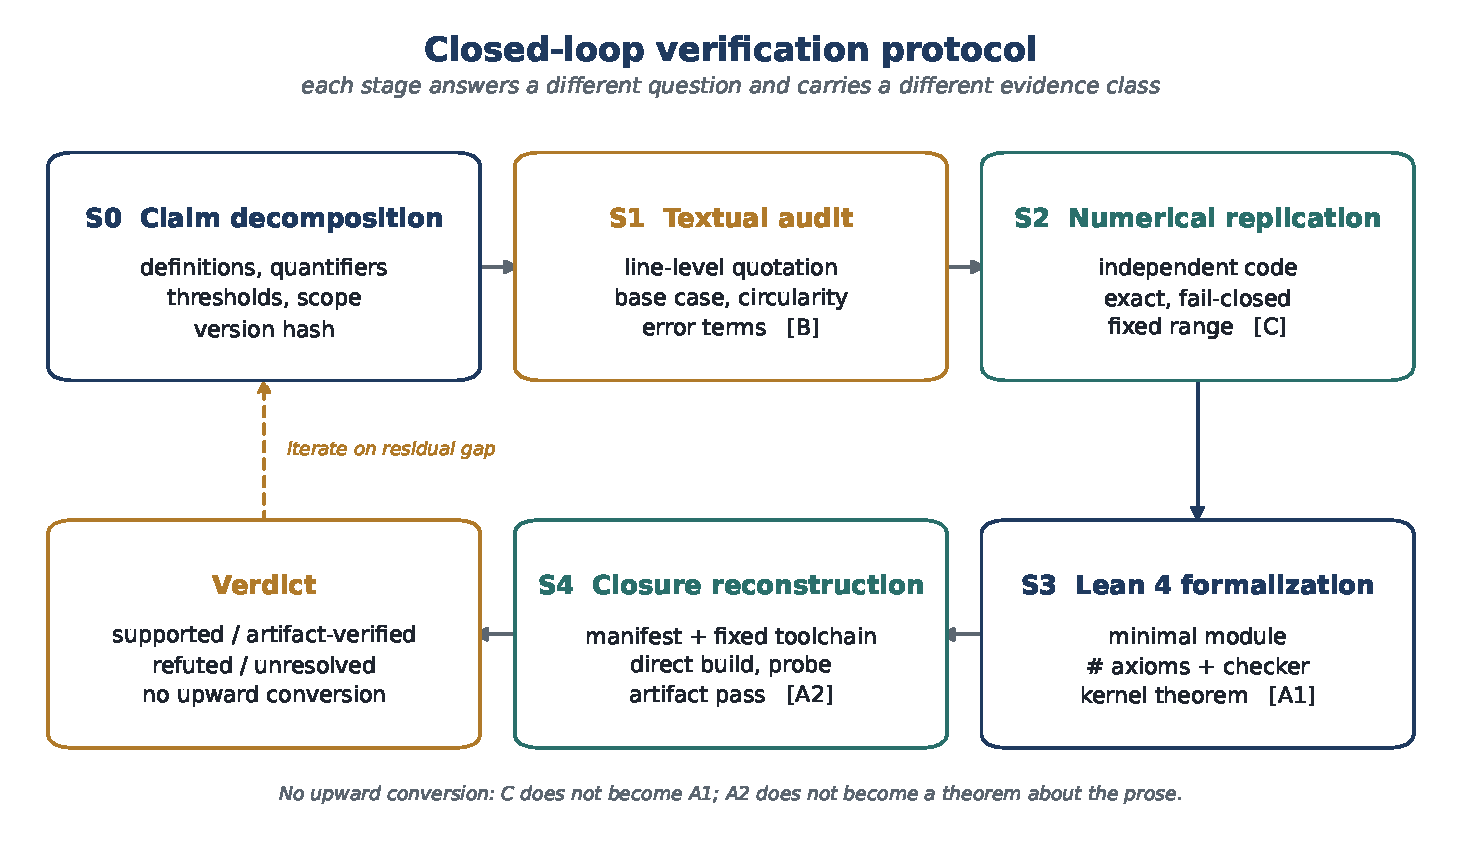
\includegraphics[width=\textwidth]{figures/fig1_pipeline.pdf}
\caption{四阶段闭环核验协议。每个阶段回答不同的问题，并产出不同等级的证据；残余的语义或范围缺口被送回 S0/S1，而不是被“通过”掩盖。}
\label{fig:pipeline}
\end{figure}

\paragraph{S0：声明分解与版本钉扎。}
把原始声明拆成定义、量词、阈值、依赖与范围五部分。对文本计算 SHA-256，对源码计算清单哈希，对工具链记录版本。输出的 claim graph 要能回答：这个声明依赖哪些定义？这些定义在原文的哪一行？阈值是“存在”还是“所有”？结论的范围是全文、某一节，还是某个形式陈述？

\paragraph{S1：逐行文本审计。}
以行号为锚，检查定义一致性、量词方向、基例、循环假设、极限与误差项、常数一致性、以及“显然”“类似地”等省略步骤。输出 B 级文本事实：每条都应是“第 $n$ 行原文 + 逻辑分析”，而不是“我觉得不对”。对关键段落，保留英文原文并给出中文译文，避免转述走样。

\paragraph{S2：可复算数值检查。}
用独立代码重算文中的恒等式、计数与数值断言。要求：范围固定、算术精确（或给出误差界）、失败即报错（fail-closed）、脚本与结果一起保存。数值检查不能证明全称命题，但可以否证一个全称的数值断言；它也可以暴露“数据不支持某个常数极限”这类经验信号。输出 C 级证据。

\paragraph{S3：Lean~4 形式化与公理审计。}
只形式化\emph{关键接口}，而不是整篇论文。关键接口通常是：一个有争议的定义、一条方向性蕴含、一个循环步骤、或一条把“正性”与“表示”连接起来的桥。形式化模块应尽量小，只依赖必要的库；用 \texttt{\#print axioms} 打印公理集，用 \texttt{leanchecker} 重放目标模块，用静态扫描排除禁忌词。输出 A1 级证据，其范围严格限于形式陈述。

\paragraph{S4：独立闭包重建。}
在源码清单、依赖清单与工具链固定的条件下，绕过原构建调度器，直接调用编译器重建目标端点的导入闭包。要求：逐模块记录退出码；只把同时存在 \texttt{.olean} 与成功标记的模块计为完成；失败即停并可恢复；最终审计同时检查源码哈希、禁忌词与产物完整性。输出 A2 级证据：它说明“这批源码在这个工具链下被内核接受”，不说明“论文的数学论证正确”。

\subsection{证据等级与判定规则}
\label{sec:evidence}

表~\ref{tab:evidence} 给出五类证据。A1 与 A2 都涉及内核，但对象不同：A1 是“某个形式陈述的证明项通过检查”，A2 是“某个源码闭包被编译且端点探针通过”。B 是文本事实，C 是有限计算，D 是判断。分类不是荣誉等级，而是\emph{适用范围}的标记：A1 并不比 B “更真”，它只是回答了另一个问题。

\begin{table}[htbp]
\centering
\small
\caption{证据等级：每一级能支持什么、不能支持什么}
\label{tab:evidence}
\begin{tabularx}{\textwidth}{@{}>{\raggedright\arraybackslash}p{0.10\textwidth}
>{\raggedright\arraybackslash}p{0.27\textwidth}
>{\raggedright\arraybackslash}X
>{\raggedright\arraybackslash}p{0.24\textwidth}@{}}
\toprule
等级 & 判据 & 能支持 & 不能支持\\
\midrule
\Aone & Lean 声明通过内核；\texttt{\#print axioms} 与 \texttt{leanchecker} 记录齐全 & 所列形式陈述在给定公理与定义下成立 & 论文原意、数学重要性、未形式化的步骤\\
\addlinespace
\Atwo & 源码哈希与清单一致；固定工具链编译完成；端点探针通过 & 该源码闭包在该工具链下被内核接受 & 论文散文、clean-room 重建、全研究范围\\
\addlinespace
\Bclass & 行号可查的原文引用 + 定义/量词/循环分析 & 具体文本缺陷、定义不一致、循环接口 & 对作者全部工作的否定、其他版本\\
\addlinespace
\Cclass & 可复算脚本 + 固定有限范围 + 精确算术/误差界 & 所列范围内的有限命题 & 无限全称命题、范围外推\\
\addlinespace
\Dclass & 专家判断、研究品味、方向性意见 & 假设、猜想、下一步 & 事实性结论\\
\bottomrule
\end{tabularx}
\end{table}

判定采用四值，而不是二值：
\begin{itemize}
\item \textbf{支持（supported）} 声明与形式陈述的语义一致，且 A1/A2 证据覆盖了声明的全部关键部分。
\item \textbf{产物通过（artifact-verified）} 工件通过检查，但声明的语义层或范围层尚未闭合；必须附带“仅限……”的限定。
\item \textbf{否证（refuted）} 声明的必要步骤被具体反例、循环或定义矛盾推翻；否证只针对所列版本与所列主张。
\item \textbf{未决（unresolved）} 现有证据不足以支持或否证；未决不是“默认为真”，也不是“默认为假”。
\end{itemize}

最重要的规则是“不得向上转换”：C 不能因为范围大而变成 A1；A2 不能因为“内核通过”而变成关于论文的定理；B 不能因为“作者没有回应”而变成普遍结论。反过来，A1 也不能因为“只是形式化”而被贬低为无意义：它恰恰能把“方向性”与“循环接口”固定下来，使争论有可检查的对象。

\subsection{停止条件与完整性门槛}
\label{sec:stops}

一个阶段只有在满足下列条件时才可停止：

\begin{itemize}
\item \textbf{文本阶段：} 关键定义、量词、基例、循环接口与误差项均已定位；每条判断都有行号；对被审文本的版本计算哈希。
\item \textbf{数值阶段：} 脚本可独立运行；范围与失败语义写明；结果与文中的断言逐项对照；反例可复算。
\item \textbf{形式阶段：} 形式模块通过编译；公理集是标准三公理的子集；无禁忌词；\texttt{leanchecker} 重放目标模块成功；形式陈述与文本定义的对应关系逐条写出。
\item \textbf{重建阶段：} 源码哈希与清单一致；所有目标模块均有产物；禁忌词扫描为 0；端点探针通过；最终状态文件把“源码身份、词法、产物完整性”三项都纳入判定。
\end{itemize}

完整性门槛不是形式主义。本文的 Wu 重建早期版本曾在缺少 690 个构建产物时仍写出 \texttt{PASS}，原因是 \texttt{missing\_build\_artifact} 只被写进 JSON，没有参与最终状态。修复后，状态要求“源码身份 + 词法 + 产物齐全”三项同时满足。这个例子说明：一个 \texttt{PASS} 的含义取决于它的判定函数；不把完整性写进判定函数，就会把“源码对”误读成“构建完成”。

\subsection{框架不做什么}
\label{sec:not-do}

本框架不替代同行评议，不证明数学猜想，不判断研究品味，也不提供“作者是否诚实”的结论。它只做一件事：把一个复合声明拆成可分别检查的部分，并记录每一部分证据的适用范围。对于本文涉及的预印本，我们只评价其文本与所列步骤，不评价作者的其他工作；对于上游形式化工程，我们只评价我们所重建的闭包，不评价其全部 4,151 个模块；对于哥德巴赫猜想本身，我们不声称任何新证明。

\section{案例一：一个“初等证明”的定义与循环}
\label{sec:paper}

\subsection{对象与版本}
\label{sec:paper-object}

被审对象是 Khaled Qazaqzeh 与 Aymen Rawashdeh 的预印本 \emph{An Elementary Proof of the Binary Goldbach Conjecture}，arXiv:2611.09007v1，2026 年 11 月 6 日，math.NT，9 页\cite{qazaqzeh}。以下行号均指 v1 的 LaTeX 源文件 \texttt{A\_Simple\_Proof\_of\_Goldbach\_Conjecture.tex}，不是 PDF 页码。该源文件的 SHA-256 为
\begin{center}
\texttt{db1fa07154ae7430245d19ac377f6d22f\\02361608014498fe3449129c3765ffd},
\end{center}
本地副本与 arXiv v1 提供的源码逐字节一致（2026 年 11 月 15 日核对）。哈希把版本钉住，读者可以脱离本文自行复核行号。

本文只评价该预印本的证明主张，不评价作者的其他工作，也不声称“论文每一步都错”。相反，我们会在下面指出其中一些正确的观察（例如 $H=K$ 的对称性；$G,H,D,K$ 是论文第 2 节定义的四个计数函数，本文不重复其定义），以示审计的边界。

\subsection{定义：非标准的 $\mathcal O$}
\label{sec:paper-def}

预印本 Definition~2.1 的第一条（源文件第 111 行）原文是：

\begin{quote}\itshape
“We say that $f$ is a big $\mathcal O$ of $g$, denoted by $\mathcal O(g)$, if
$\lim_{n\to\infty} f(n)/g(n)=c$ for some nonzero real number $c$.”
\end{quote}

\noindent 译文：若存在非零实数 $c$，使得 $f(n)/g(n)\to c$，则称 $f$ 是 $g$ 的大 $\mathcal O$。

标准的大 $\mathcal O$ 只要求存在常数 $C$，使得最终 $|f(n)|\le C g(n)$；它允许比值为 $0$，也允许比值不存在。预印本的定义要求比值\emph{收敛到一个非零常数}，这是一个强得多的双侧渐近条件。按这个定义，“$G(2n)=\mathcal O(n/\ln^2 n)$”意味着
\begin{equation}
\lim_{n\to\infty}\frac{G(2n)\ln^2(2n)}{n}=c\ne0.
\label{eq:paperO}
\end{equation}
其中 $G(2n)$ 是 $2n$ 的（有序）哥德巴赫表示数。定理~1.1 的陈述写的是 $\ln^2 n$，而证明第 182/184 行用的是 $\ln^2(2n)$；由于 $(\ln(2n)/\ln n)^2\to1$，非零极限不受影响。本文的形式化采用证明中出现的 $\ln^2(2n)$ 形式。

\subsection{两难：字面读法与标准读法}
\label{sec:dilemma}

对第 111 行的定义，有两种读法。两种读法都不能支撑论文的证明主张。

\paragraph{读法 A（字面读法）。}
若严格按第 111 行，定理~1.1 不是“上界”，而是一个带非零常数的渐近下界。由 $G(2n)\ge0$ 可得 $c\ge0$；由 $c\ne0$ 得 $c>0$；于是最终 $G(2n)>0$，即每个充分大的偶数都是两个素数之和。也就是说，\emph{在这个定义下，定理~1.1 已经蕴含 $1+1$}。这不是说定理~1.1 被证明了，而是说它的陈述本身已经包含了结论；如果证明又把这个结论当作假设，就构成循环。下一小节给出形式化定理，第~\ref{sec:circularity} 节给出行号证据。

\paragraph{读法 B（标准读法）。}
若作者本意是标准大 $\mathcal O$（只要求上界），那么定理~1.1 不再蕴含 $G(2n)>0$；一个恒为零的计数函数也满足上界。此时，证明中从“$G(2n-2)=\mathcal O(n/\ln^2 n)$”推出“$G(2n-2)>0$”或“$\alpha<2$”的步骤失去依据。论文没有给出替代的正性论证。因此，按标准读法，证明同样不能成立，只是失败的位置从“循环”变成了“关键正性步骤缺失”。

\paragraph{结论。}
两种读法下，论文都没有建立起“每个大偶数是两个素数之和”。字面读法暴露的是陈述层面的自我包含与证明层面的循环；标准读法暴露的是关键估计的缺失。这个两难比单独指出“$\mathcal O$ 定义不标准”更强：它说明问题不在于某个符号的用法，而在于定理、证明与结论之间的逻辑接口。

\subsection{形式化：定理~1.1 蕴含 $1+1$}
\label{sec:paper-formal}

令
\begin{equation}
\g(N):=\#\{p\le N:\ p\ \text{素数}\land N-p\ \text{素数}\}.
\label{eq:count}
\end{equation}
$\g$ 把每个满足条件的 $p$ 计一次，因此是有序表示数（对角情形只计一次）。对 $N\ge6$，$p=2$ 不会贡献，因为 $N-2$ 是大于 $2$ 的偶数，必为合数；所以在相关范围内 $\g(2n)$ 与论文的 $G(2n)$ 一致。把论文定理~1.1 在其自身 $\mathcal O$ 定义下的内容形式化为
\begin{equation}
\PaperTheorem:\quad \exists c\in\R,\ c\ne0,\quad
\lim_{n\to\infty}\frac{\g(2n)\ln^2(2n)}{n}=c.
\label{eq:papertheorem}
\end{equation}

\begin{theorem}[论文定理的自我包含]
\label{thm:paper-implies-bg}
$\PaperTheorem\Longrightarrow\BG$。
\end{theorem}

\begin{proof}
设 $a_n:=\g(2n)\ln^2(2n)/n$。由 $\PaperTheorem$，$a_n\to c\ne0$。

\begin{enumerate}[label=(\roman*)]
\item 因为 $\g(2n)\ge0$、$\ln^2(2n)\ge0$、$n>0$，所以最终 $a_n\ge0$，从而 $c\ge0$。
\item 由 $c\ne0$ 得 $c>0$。
\item 因为 $a_n\to c>0$，所以最终 $a_n>0$。对这些 $n$，$\ln^2(2n)>0$ 且 $n>0$，故 $\g(2n)>0$。
\item $\g(2n)>0$ 意味着存在素数 $p,q$ 使 $2n=p+q$。因此每个充分大的偶数都是两个素数之和，即 $\BG$。
\end{enumerate}
\end{proof}

在 Lean~4 中，该定理名为 \texttt{paperTheorem\_implies\_binaryGoldbach}，与另外 7 条定理一起位于 \texttt{Goldbach/Gap.lean}，公理集为标准三公理；第~\ref{sec:endpoints} 节给出完整的验证记录。这个定理只说明“按字面定义，定理~1.1 蕴含 $1+1$”，不说明“论文证明了定理~1.1”，更不说明“哥德巴赫猜想被证明”。它把争论的焦点从“$\mathcal O$ 是不是写错了”转移到“证明是否真的建立了这个陈述”。

\subsection{循环在哪里}
\label{sec:circularity}

一个强的定理陈述还不是循环证明；循环在证明的开头。预印本源文件第 180 行原文是（强调为引者所加；交叉引用已渲染为编号）：

\begin{quote}\itshape
“We proceed by induction on $n$ to verify the claim of the theorem. Thus we can assume that
$G(2n-2)$ \textbf{and} $G(2n)$ are $\mathcal O\bigl(n/\ln^{2} n\bigr)$ functions as a
consequence of the result of Lemma (note). As a consequence of Equation (1), the induction
hypothesis on the antidiagonals $I_{2n-2}$, \textbf{the positivity of $G(2n-2)$} and the
result of Lemma (note), we conclude \ldots”
\end{quote}

\noindent 译文：我们对 $n$ 作归纳来验证定理。于是可以假设 $G(2n-2)$ \textbf{与} $G(2n)$ 都是 $\mathcal O(n/\ln^2 n)$ 函数……由式~(1)、对反对角线 $I_{2n-2}$ 的归纳假设、\textbf{$G(2n-2)$ 的正性}以及引理，我们推出……

按字面读，这段话把 $G(2n)$——当前要证的情形——列入了“可以假设”的对象。归纳假设只应给出 $n-1$ 的情形 $G(2n-2)$；若要从 $G(2n-2)$ 推出 $G(2n)$，需要一个独立的递推论证，而论文没有给出。同一句还把 $G(2n-2)>0$ 当作输入。这一点单独处理，不并入循环结论：在字面定义下，“$G(2n-2)=\mathcal O(n/\ln^2 n)$”已经蕴含最终 $G(2n-2)>0$，因此已预设结论所要求的正性（B）；在标准读法下，该正性步骤则失去依据。第 184 行又从同一 $\mathcal O$ 陈述推出 $\alpha<2$；若 $G(2n-2)\sim c\,n/\ln^2 n$，则 $\alpha=2-c$，$\alpha<2$ 等价于 $c>0$，仍是同一个正性。

因此，循环的准确表述有两层；此外还有一个不并入循环的正性读法问题：

\begin{itemize}
\item \textbf{机器检查的部分：} 在字面 $\mathcal O$ 定义下，定理~1.1 蕴含 $\BG$（定理~\ref{thm:paper-implies-bg}）。
\item \textbf{文本比对的部分：} 第 180 行按字面把 $G(2n)$ 本身列入假设，这是循环证据；就循环而言，该归纳步骤假设了所要证明的当前情形。
\item \textbf{正性读法的独立部分：} 同一句把 $G(2n-2)>0$ 当作输入；在字面定义下，这已预设结论的正性（B），在标准读法下则缺乏依据。此项不作为循环证据。
\end{itemize}

这两层证据等级不同（A1 与 B），不能混写。我们不说“Lean 证明了论文循环”；Lean 证明的是一个条件蕴含，循环的判断来自对第 180 行的逐字阅读。把两者分开，是本文证据分级的一个具体应用。

\subsection{其他文本与数值问题}
\label{sec:paper-other}

除循环外，审计还发现以下问题。它们不是“全文皆错”的证据，但各自独立地削弱了论文的可靠性。

\paragraph{没有基例。}
归纳论证没有给出起点。即使每一步递推成立，也需要至少一个 $n_0$ 使 $G(2n_0)>0$；论文没有明确给出。对哥德巴赫这类“充分大”命题，基例可以由有限验证补上，但论文没有引用或构造这样的基例。

\paragraph{$R_1$ 的断言不受归纳假设控制。}
论文第 222 行附近说，由归纳假设可以假设 $R_1=o(n/\ln^2 n)$。但 $R_1$ 数的是四点构型（涉及“三个素数 + 一个合数”的元组），它与 $G$ 的计数不是同一个对象；$G$ 的界不能控制 $R_1$。这句话不是推导，而是把最难的估计重新命名后当作假设。即使该估计为真，论文也没有证明它。

\paragraph{常数一致性未证。}
证明中 $\alpha$ 在每一步可能变为 $\alpha-\beta$ 等；论文没有证明这些常数在整个归纳过程中保持一致、不会最终变负。把“$\approx$”当等号使用，也使误差可能逐步累积；论文没有给出累积误差的界。

\paragraph{式~(1)(2) 各差 1，方向相反。}
这是可以独立复算的硬错误。独立脚本对 $3\le x\le6000$ 的每个整数重算，得到
\begin{align}
G(2x)+H(2x)&=\pi(2x-3)-1, \label{eq:true1}\\
D(2x)+K(2x)&=x-1-\pi(2x-3), \label{eq:true2}
\end{align}
而论文写的是 $\pi(2x-3)$ 与 $x-2-\pi(2x-3)$。两处偏差方向相反：式~(1) 多 $1$，式~(2) 少 $1$。表~\ref{tab:numerical} 给出 $x=10$ 的实例：$G=4$，$H=2$，$D=0$，$K=2$，$\pi(17)=7$，故 $G+H=6$ 而论文公式给 $7$；$D+K=2$ 而论文公式给 $1$。

\begin{table}[htbp]
\centering
\small
\caption{式~(1)(2) 的独立重算（$x=10$，$2x=20$）}
\label{tab:numerical}
\begin{tabular}{@{}lccc@{}}
\toprule
量 & 论文公式 & 独立重算 & $x=10$ 的值\\
\midrule
$G+H$ & $\pi(2x-3)$ & $\pi(2x-3)-1$ & $6$（论文公式给 $7$）\\
$D+K$ & $x-2-\pi(2x-3)$ & $x-1-\pi(2x-3)$ & $2$（论文公式给 $1$）\\
\bottomrule
\end{tabular}
\end{table}

该差异对 $3\le x\le6000$ 的每个 $x$ 都成立，不是个别边界情形。它说明论文的组合计数至少有一处系统性偏移；这类偏移在归纳中被反复使用，可能累积，但本文不声称它单独构成对全文的否证。它与循环、缺失基例、未控制的 $R_1$ 一起，构成“证明未建立”的充分理由。

\paragraph{推论的范围错误。}
论文的一条推论说“任意奇数都是三个奇素数之和”，但 $5$ 与 $7$ 不是（最小的三个奇素数之和是 $3+3+3=9$）。正确表述应是“充分大的奇数”。这是一个小错误，但它与全文“充分大”量词处理不严谨的模式一致。

\paragraph{数值上不支持常数极限。}
用独立脚本计算 $G(2n)\ln^2(2n)/(2n)$，在 $2n\approx4.1\times10^6$ 附近可因 $2n$ 的素因子结构从约 $1.52$ 跳到约 $6.32$；差异来自 Hardy--Littlewood 奇异级数，而不是一个常数。数值不能严格证明“极限不存在”，但它足以说明论文的常数极限断言没有得到数据的支持。该预印本的图~2 之所以看起来接近 $1$，是因为它除以了奇异级数，而不是除以一个常数。这一点是 C 级证据，只作为辅助。

\subsection{判定与边界}
\label{sec:paper-verdict}

对 arXiv:2611.09007v1 的判定是：\textbf{其证明主张被否证}，但这是对“该版本、该证明”的否证，不是对哥德巴赫猜想的否证，也不是对作者全部工作的否定。具体地说：

\begin{itemize}
\item 按字面 $\mathcal O$ 定义，定理~1.1 蕴含 $1+1$（A1），而第 180 行把当前情形 $G(2n)$ 列入归纳假设（B），构成循环；同一句把 $G(2n-2)>0$ 当作输入，在字面定义下已预设结论的正性（B），在标准读法下则失去依据；
\item 按标准 $\mathcal O$ 读法，关键正性步骤失去依据（B），论文没有替代论证；
\item 式~(1)(2) 在 $3\le x\le6000$ 上各差 $1$、方向相反（C），且没有基例、$R_1$ 断言未证、常数一致性未证（B）；
\item 因此，论文没有建立其标题所声称的结论。
\end{itemize}

如果作者发布 v2，或对第 111 行的定义作出不同解释，本文的结论应重新对照 v2 复核；我们保留“针对 v1”的限定，不把 v1 的问题自动迁移到 v2。若作者认为我们误读了某一行，最有效的回应是指出具体行号与替代推导；本文的所有引用都绑定了源码哈希，讨论可以逐行进行。

\section{案例二：把端点的弱性搬进 Lean}
\label{sec:endpoints}

\subsection{形式设置}
\label{sec:endpoints-setting}

我们在 Lean~4.33.0-rc1 + Mathlib 下工作，使用上游 \texttt{goldbach-lean} 的 \texttt{Goldbach.Statement} 中的 \texttt{BinaryGoldbach} 定义，以及三个端点的字面形状。为保持最小依赖，新增模块 \texttt{Goldbach/Gap.lean} 只导入 \texttt{Goldbach.Statement} 与 Mathlib，不导入 1,800 余个筛法模块；这样，端点方向性的检查不依赖大工程的构建状态。检查文件 \texttt{Goldbach/GapChecks.lean} 打印每条定理的类型与公理集；\texttt{Goldbach/GapLiveChecks.lean} 则用活的 Li--Liu 端点直接证出形状定义，确认形状不是从日志手抄的。

形式陈述与第~\ref{sec:bg} 节的定义一致。为便于阅读，下面用自然语言重述，Lean 名称在表~\ref{tab:eight} 中给出。

\begin{theorem}[$1+1\Rightarrow$ Chen]
\label{thm:bg-chen}
$\BG\Longrightarrow\Chen$。
\end{theorem}
\begin{proof}
设 $N\ge N_0$ 为偶数，且 $N=p+q$，$p,q$ 为素数。取 Chen 陈述中的同一个 $p$ 与 $q$；$q$ 是素数，当然满足“素数或两个素数之积”。阈值不变。
\end{proof}

\begin{theorem}[$1+1\Rightarrow$ Li--Liu]
\label{thm:bg-ll}
$\BG\Longrightarrow\LL$。
\end{theorem}
\begin{proof}
取阈值为 $\max(N_0,4)$，并令 $r=1$。则 $N=p+1\cdot q$；$r=1$ 满足“$r=1$ 或 $r$ 为素数”；$1^{10}=1\le q^9$ 因为 $q\ge2$。
\end{proof}

\begin{theorem}[$1+1\Rightarrow$ Wu]
\label{thm:bg-wu}
$\BG\Longrightarrow\WU$。
\end{theorem}
\begin{proof}
取阈值为 $\max(N_0,512)$，并令 $r=1$。则 $N=p+1\cdot q$，$r=1$ 合法，且 $1^{5000}=1\le q^{4469}$。
\end{proof}

这三条证明在数学上是平凡的；把它们形式化的意义不在于难度，而在于把“方向”固定为可检查的对象。公众叙事中的“$1+2$ 离 $1+1$ 只差一点”很容易滑向“$1+2$ 可以推出 $1+1$”；三条定理把相反的箭头写进了内核。

\subsection{八条定理与三条见证}
\label{sec:eight}

表~\ref{tab:eight} 列出 8 条定理。前三条是上面的方向性蕴含；第 4--6 条是“表示谓词严格更宽”的见证；第 7 条是计数与表示之间的桥；第 8 条是案例一的机器版本。

\begin{table}[htbp]
\centering
\small
\caption{8 条经 Lean~4 内核检查的定理}
\label{tab:eight}
\begin{tabularx}{\textwidth}{@{}c
>{\raggedright\arraybackslash}p{0.36\textwidth}
>{\raggedright\arraybackslash}X c@{}}
\toprule
\# & Lean 名称 & 陈述（摘要） & 等级\\
\midrule
1 & \texttt{binaryGoldbach\_implies\_}\newline\texttt{chen} & $1+1\Rightarrow$ Chen $1+2$ & A1\\
2 & \texttt{binaryGoldbach\_implies\_}\newline\texttt{onePlusOneNine} & $1+1\Rightarrow$ Li--Liu $1+1.9$ & A1\\
3 & \texttt{binaryGoldbach\_implies\_}\newline\texttt{onePlusOne8938} & $1+1\Rightarrow$ Wu $1+1.8938$ & A1\\
4 & \texttt{chen\_second\_summand\_class\_}\newline\texttt{includes\_composite} & Chen 允许合数第二加数（$4=2\cdot2$） & A1\\
5 & \texttt{liu\_multiplier\_class\_}\newline\texttt{includes\_nontrivial} & Li--Liu 允许 $r=3\ne1$（$18=3+3\cdot5$） & A1\\
6 & \texttt{wu\_multiplier\_class\_}\newline\texttt{includes\_nontrivial} & Wu 允许 $r=2\ne1$（$13=7+2\cdot3$） & A1\\
7 & \texttt{goldbachCount\_pos\_iff} & $0<\g(N)$ 当且仅当 $N$ 是两个素数之和 & A1\\
8 & \texttt{paperTheorem\_implies\_}\newline\texttt{binaryGoldbach} & 论文定理（其自身 $\mathcal O$）$\Rightarrow1+1$ & A1\\
\bottomrule
\end{tabularx}
\end{table}

第 4--6 条见证值得展开。它们不是说“存在一个数不能用两个素数表示”，而是说端点的\emph{表示谓词}比“两个素数之和”更宽：

\begin{itemize}
\item Chen：$4=2\cdot2$，第二个加数 $q=4$ 是合数，却满足“素数或两个素数之积”。注意 $4$ 本身是 $2+2$，所以这不是一个反例数，而是一个反例\emph{表示}。
\item Li--Liu：$18=3+3\cdot5$，$r=3\ne1$，$3^{10}\le5^9$，$p=3$、$q=5$ 为素数。$18$ 本身也是 $5+13=7+11$，所以这同样不是反例数。
\item Wu：$13=7+2\cdot3$，$r=2\ne1$，$2^{5000}\le3^{4469}$；$13$ 本身也是 $2+11$。
\end{itemize}

这些见证只说明谓词更宽，\emph{不是}独立性证明。要证明“端点不能推出 $1+1$”需要元数学论证；本文没有给出，也不假装给出。我们在措辞上严格区分“表示谓词更宽”与“端点不蕴含 $1+1$”。前者是 A1，后者是未决。

第 7 条桥接定理是
\begin{equation}
0<\g(N)\iff \exists p,q\in\N,\ p,q\ \text{素数}\land N=p+q.
\label{eq:bridge}
\end{equation}
它把“计数为正”与“存在表示”连接起来，是第 8 条定理的最后一步。第 8 条已在第~\ref{sec:paper-formal} 节给出数学证明；其 Lean 名称是 \texttt{paperTheorem\_implies\_binaryGoldbach}。

\subsection{端点层级}
\label{sec:hierarchy}

除上述 8 条外，补充模块 \texttt{Goldbach/EndpointHierarchy.lean} 还机器检查了端点之间的强弱关系。其核心是一个初等的指数比较：

\begin{proposition}[Wu $\Rightarrow$ Li--Liu]
\label{prop:wu-ll}
对 $r,q\in\N$，若 $q\ge1$ 且 $r^{5000}\le q^{4469}$，则 $r^{10}\le q^{9}$。
\end{proposition}
\begin{proof}
若 $r=0$，则 $r^{10}=0\le q^9$。若 $r\ge1$，由 $r^{5000}\le q^{4469}$ 得
\[
(r^{10})^{500}=r^{5000}\le q^{4469}\le q^{4500}=(q^9)^{500}.
\]
由于 $x\mapsto x^{500}$ 在非负整数上严格递增，故 $r^{10}\le q^9$。
\end{proof}

于是 Wu 端点（在相同或更大的阈值下）蕴含 Li--Liu 端点；而 Li--Liu 端点蕴含 Chen 端点，因为 $r=1$ 时 $rq=q$ 是素数，$r$ 为素数时 $rq$ 是两个素数之积。合并起来就是
\[
\BG\Longrightarrow\WU\Longrightarrow\LL\Longrightarrow\Chen.
\]
据项目日志，这条链的每一段都有 Lean 检查（补充模块中 5 条定理，公理集同为标准三公理）；本文不把它们计入 8 条主定理，但把它们作为端点层级的辅助证据。它说明三个端点不是彼此独立的“三个几乎证明”，而是一条严格递减的强度链；链的起点是 $1+1$，终点是 $1+2$，方向不能反转。

\subsection{验证记录与解释}
\label{sec:endpoints-verification}

8 条主定理的验证记录如下：

\begin{itemize}
\item 每条 \texttt{\#print axioms} 的公理集都包含于 $\{\texttt{propext},\texttt{Classical.choice},\texttt{Quot.sound}\}$，没有 \texttt{sorryAx}、没有自定义公理；
\item 静态扫描剥离注释与字符串后，\texttt{sorry} / \texttt{admit} / \texttt{axiom} / \texttt{native\_decide} / \texttt{unsafe} / \texttt{skipKernelTC} 均为 0 命中；
\item \texttt{leanchecker} 重放 \texttt{Goldbach.Gap} 返回 0；
\item 活端点检查 \texttt{live\_one\_plus\_one\_nine\_has\_shape} 直接由 \texttt{Goldbach.one\_plus\_one\_nine} 证出 \texttt{OnePlusOneNineShape}，说明 Li--Liu 形状与活端点定义相等，而不是手抄；
\item 静态检查（当时本地树 1,806 个源模块）报告 \texttt{issues} 为空；后续新增文件后计数变为 1,808/1,812，属于快照差异，不影响本模块的独立性。
\end{itemize}

这些结果的解释需要克制。它们是 A1 级：只说明 8 条形式陈述在标准公理下成立。它们不证明 Chen、Li--Liu 或 Wu 的原始论文，不证明这些端点的数学定理在文献意义上已被独立验证，也不证明哥德巴赫猜想。它们能做的是：把“端点弱于 $1+1$”从口头共识变成可重放的命题，并为案例一提供一个精确的机器接口。

\subsection{判定}
\label{sec:endpoints-verdict}

对“$1+1$ 蕴含三个端点”与“三个端点的表示谓词严格更宽”的判定是\textbf{支持（A1）}；对“端点可以推出 $1+1$”的判定是\textbf{未决}，且现有材料没有给出这样的推导。对“8 条定理是新的深刻数学”的判定是否定的：它们中的大多数是定义展开与初等指数比较，其价值在形式化与审计，而不在数学发现。我们在第~\ref{sec:reflexive} 节对此作进一步反思。

\section{案例三：Wu 端点导入闭包的独立重建}
\label{sec:wu}

\subsection{对象与范围}
\label{sec:wu-object}

上游 \texttt{subfish-zhou/goldbach-lean} 的研究子工程 \texttt{research/wu2008/} 沿 Wu04/Wu08 双筛路线，形式化出端点
\begin{equation}
\begin{aligned}
\WU:\quad &\exists T\ge512,\ \forall N\ge T,\ \Even(N)\Longrightarrow
\exists p,r,q\in\N,\ p,q\ \text{素数}\ \land\\
&(r=1\lor r\ \text{素数})\land N=p+rq\land r^{5000}\le q^{4469}.
\end{aligned}
\label{eq:wu}
\end{equation}
其最终证明位于 \texttt{src/WR2ClassicalCertificate.lean}，公开声明为 \texttt{WuPaper.ClassicalSlots.one8938}。截至 2026 年 11 月 16 日，以 \texttt{all:"1.8938"} 检索 arXiv 返回 0 条；外部可核的对象是上游形式化仓库，而不是一篇公开的 Wu 论文。这一点很重要：我们重建的是\emph{形式化产物}，不是一篇论文的同行评议状态。

上游声称的研究范围是 4,151 个模块，最终定理的导入闭包是 3,764 个模块，约 525,529 行有效代码、621,451 行物理行；其验收口径是 3,500 个实际编译收据加 651 个未变依赖\cite{upstream}。本文只重建 3,764 个导入闭包，不重建 4,151 个全研究范围；因此下文所有“全部”都指“全部 3,764 个闭包模块”，不是“全部上游工作”。

端点源文件的 LF 归一化 SHA-256 为
\begin{center}
\texttt{ccd260b66cdd786b22d6b81e6fffe966\\bd57efc45c2370d95aed3f5b2d8c0804},
\end{center}
与 \texttt{source-manifest.json} 的记录一致。本地仓库 HEAD 为 \texttt{c73fce1}（上游 \texttt{9d4c3a4} 之后的本地提交），端点源码与清单、上游 \texttt{main} 三者逐字节一致（只差 CRLF）。这把“我们编的是哪批字节”钉住了。

\subsection{重建协议}
\label{sec:wu-protocol}

重建使用 \texttt{build\_wu.py}，不经过 Lake 调度器，直接调用固定的 Lean~4.33.0-rc1 的 \texttt{lean.exe}。这里的“独立”指构建路径独立于上游 Lake 调度器、由本文管线直接调用固定工具链；它不是第三方独立复现，也不是 clean-room 重建。关键设置如下：

\begin{itemize}
\item 每个 Lean 进程 \texttt{-j1}，并加 \texttt{-DwarningAsError=true}；\texttt{W*} 与 \texttt{R2*} 模块另加 \texttt{-DautoImplicit=false}；
\item 4 个 worker；源码 $\ge120$ KB 的重模块最多 2 个同时编译（\texttt{--big-kb 120 --big-slots 2}），以避免内存峰值叠加；
\item 只认同时存在 \texttt{.olean} 与成功标记 \texttt{.ok} 的模块为完成；失败即停，可从 \texttt{.ok} 热恢复；
\item 构建前先做源码身份检查：3,764/3,764 个 LF 归一化 SHA-256 与 \texttt{source-manifest.json} 一致；
\item 构建后做词法审计：剥离注释与字符串后，\texttt{sorry}/\texttt{admit}/自定义 \texttt{axiom}/\texttt{native\_decide}/\texttt{unsafe}/\texttt{skipKernelTC} 必须为 0；
\item 端点探针：编译 \texttt{WR2ClassicalCertificate} 的检查文件，打印 6 条声明的公理集；再用 \texttt{leanchecker} 重放端点模块。
\end{itemize}

构建由一个脱离 agent 会话的 supervisor 托管。此前多次续跑因会话结束、进程被收走而中断；本轮用 WMI 启动 \texttt{cmd.exe}，使 supervisor 的父进程不在 agent 进程树内，从而在会话结束后继续运行。supervisor 负责：续跑构建、在硬崩溃时把 worker 从 4 降到 3、完成后自动运行闭包审计与端点检查、写最终状态文件。这不是数学方法，但它是长任务可复现性的一部分：如果构建进程随会话消失，再好的脚本也无法给出完整结果。

\subsection{结果}
\label{sec:wu-results}

表~\ref{tab:wu} 汇总重建结果。图~\ref{fig:progress} 给出从 2026 年 11 月 16 日 13:47 到 11 月 17 日 02:00 的累计进度快照。

\begin{table}[htbp]
\centering
\small
\caption{ Wu 端点导入闭包的独立重建结果（2026-11-17 02:01，UTC+8）}
\label{tab:wu}
\begin{tabularx}{\textwidth}{@{}>{\raggedright\arraybackslash}p{0.24\textwidth}
>{\raggedright\arraybackslash}X
>{\raggedright\arraybackslash}p{0.25\textwidth}@{}}
\toprule
项目 & 结果 & 证据\\
\midrule
研究范围 & 4,151 模块（上游口径，未全建） & 上游 README\\
导入闭包 & 3,764 模块 & \texttt{STATUS.json}\\
源码身份 & 3,764/3,764 LF SHA-256 与清单一致 & \texttt{closure\_audit.json}\\
源码体量 & 30,215,769 字节；621,451 物理行 & 同上\\
词法禁忌 & 0 命中 & 同上\\
构建完成 & 3,764/3,764；0 真实失败 & \texttt{STATUS.json}\\
本段构建 & 617 模块；6,479.7 秒；4 worker & 同上\\
端点探针 & 6 条声明；公理集恰为标准三公理 & \texttt{final\_probe.log}\\
\texttt{leanchecker} & 端点模块 rc 0；37.5 秒 & \texttt{FINAL\_STATUS.json}\\
端点 \texttt{.olean} & SHA-256 \texttt{6e8702bd\ldots}；20,192 字节 & 同上\\
clean-room & 否；\texttt{.ok} 跨会话复用 & 构建记录\\
4,151 全范围 & 否 & 范围声明\\
论文散文 & 未验证 & 方法边界\\
\bottomrule
\end{tabularx}
\end{table}

\begin{figure}[htbp]
\centering
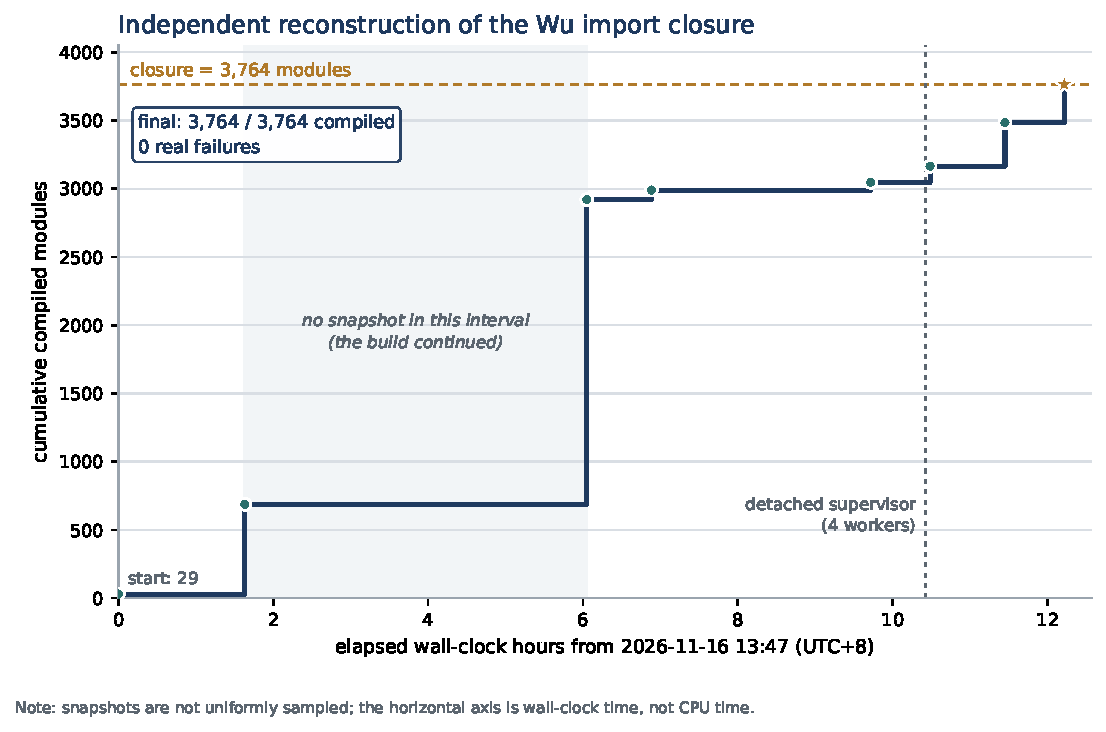
\includegraphics[width=\textwidth]{figures/fig2_progress.pdf}
\caption{ Wu 导入闭包的累计编译进度。横轴是墙钟时间，不是 CPU 时间；快照并非均匀采样，平缓段不代表构建停止。最终 3,764/3,764，0 真实失败。}
\label{fig:progress}
\end{figure}

端点探针的输出是 6 行，全部为
\begin{center}
\texttt{depends on axioms: [propext, Classical.choice, Quot.sound]}.
\end{center}
{\raggedright
6 条声明分别是 \texttt{WuLegacyLiteralAcceptance}、\texttt{WuPaper.ClassicalSlots.one8938}、\texttt{WuLiteralAcceptance}、\texttt{WuLiveShapeCheck}、\texttt{WuPaper.ClassicalSlots.one894}、\texttt{WuPaper.ClassicalSlots.classical\_lower}。其中 \texttt{WuLiteralAcceptance} 用手写的字面类型直接由 \texttt{one8938} 证出，\texttt{WuLiveShapeCheck} 由同一端点证出 \texttt{Goldbach.OnePlusOne8938Shape}，说明端点的字面类型与形状定义相等。端点自身的编译日志也打印了 \texttt{one8938}、\texttt{one894} 与 \texttt{classical\_lower} 的标准三公理。
\par}

\subsection{它证明了什么、没有证明什么}
\label{sec:wu-scope}

\textbf{它证明了：} 在固定源码、固定依赖、固定工具链下，3,764 个导入闭包模块都被本管线至少编译过一次，且没有真实失败；源码哈希与清单一致；没有禁忌词；端点声明通过内核检查，公理集恰为标准三公理；端点模块通过 \texttt{leanchecker} 重放。用一句话说：\emph{该端点闭包在本工作区被独立重建，并通过产物级内核检查。}

\textbf{它没有证明：}
\begin{enumerate}
\item \textbf{不是 clean-room 重编。} \texttt{.ok} 标记跨会话复用；最后一段是在已有 3,147 个产物的基础上续编 617 个模块。每个模块都被本管线编译过一次，但不是“清空 \texttt{lib} 后一次跑完”。因此它不能排除“早期产物与当前源码不一致”的极端情况；源码哈希一致与逐模块日志降低了这一风险，但没有把它降为零。
\item \textbf{没有重放 3,764 个模块。} \texttt{leanchecker} 只重放 \texttt{WR2ClassicalCertificate} 一个模块的新声明；它不重放所有导入模块，也不是第二个独立内核。准确说法是“端点模块通过内核重放”，不是“整个闭包通过独立内核重放”。
\item \textbf{没有构建 4,151 个全研究范围。} 本地只构建了 3,764 个导入闭包；上游的 3,500 个编译收据加 651 个未变依赖是上游口径，不是本文的独立验证。
\item \textbf{没有验证论文散文。} 内核检查的是 \texttt{src/} 里的 Lean 源码；论文中“为什么这些槽位成立”的数学论证不在内核检查范围内。形式陈述与论文语义的逐行一致性也没有机器证明。本文能说的是“形式化端点通过检查”，不是“Wu 的论文被验证”。
\item \textbf{没有改变 12 项任务账本。} 上游 \texttt{mathematical-status.json} 的 12 项任务仍全部 \texttt{global\_complete: false}；本文的构建不改变那本账。顶层布尔值与任务账本之间的张力见下一小节。
\end{enumerate}

\subsection{范围账本与文本张力}
\label{sec:wu-tension}

上游的验收材料存在两处需要在引用时说明的张力。

{\raggedright
第一，\texttt{mathematical-status.json} 顶层写 \texttt{global\_theorem\_proved: true}、\texttt{global\_wu1894\_theorem\_complete: true}、\texttt{final\_acceptance.status: pass}，但同一文件的 \texttt{tasks[]} 中 12 项全部 \texttt{global\_complete: false}。如果 12 项是“Wu04/Wu08 源路线恢复”的 campaign 账本，而最终端点走的是 \texttt{WR2Classical*} 证书路线，那么两者可以并存；但文件本身没有一句话解释这个切换。如果 12 项被视为终点的必经步骤，则顶层为真与任务全假直接冲突。本文不替上游解释这一张力；我们只报告它，并建议引用时写明“是哪一本账”，不要只引顶层布尔值。
\par}

{\raggedright
第二，\texttt{completion-audit.json} 标注 \texttt{reviewed\_at\_utc: 2026-10-24}，其 scope 只写到 $1+1.894$，并明确写“No separate literal acceptance of 1.8938 is claimed.”；而 10 月 26 日之后的 \texttt{docs/VERIFICATION.md} 与研究 README 已改称 $1.8938$ 验收通过。两者不是同一时点，不能拿 10 月 24 日的 audit 当 current，也不能用 10 月 26 日的 README 反推 audit 已更新。本文的独立重建发生在 2026 年 11 月 17 日，在 \texttt{gap-v0.1.2} 中属于 postseal 补充证据，不修改该版 68 文件包；本版 \texttt{gap-v0.1.3} 将其纳入封存清单（79 文件），旧版保持原样，也不把新结论回写成封存时点的内容。
\par}

这些张力不影响“3,764 个闭包模块被本地编译”这一事实，但影响“上游验收到底覆盖了什么”的解释。把它们写出来，是闭环核验的一部分：一个只报告 \texttt{PASS}、不报告账本张力的审计，仍然是不完整的。

\subsection{判定}
\label{sec:wu-verdict}

对“Wu 端点的 3,764 导入闭包在本地被独立重建并通过产物级内核检查”的判定是\textbf{产物通过（A2）}，范围限定为：本工作区、固定工具链、3,764 个导入闭包、非 clean-room、端点模块级重放。对“Wu 的论文在数学上被验证”的判定是\textbf{未决}；对“哥德巴赫猜想被证明”的判定是\textbf{否证}（就本文所审材料而言，没有任何无条件定理以 $\BG$ 为结论）。对“4,151 个模块全部构建”的判定是\textbf{未决}，因为本文没有做。

\section{综合讨论}
\label{sec:synthesis}

\subsection{声明矩阵}
\label{sec:matrix}

表~\ref{tab:matrix} 把本文涉及的主要声明、方法、证据等级、判定与残余风险放在一起。它是全文的浓缩：每个“是/否”都带一个范围，每个范围都带一个证据等级。

\begin{table}[htbp]
\centering
\footnotesize
\caption{主要声明的证据矩阵}
\label{tab:matrix}
\begin{tabularx}{\textwidth}{@{}c
>{\raggedright\arraybackslash}p{0.25\textwidth}
>{\raggedright\arraybackslash}p{0.10\textwidth}
>{\raggedright\arraybackslash}p{0.09\textwidth}
>{\raggedright\arraybackslash}p{0.16\textwidth}
>{\raggedright\arraybackslash}X@{}}
\toprule
ID & 声明 & 方法 & 等级 & 判定 & 残余/范围\\
\midrule
C0 & 预印本证明了哥德巴赫猜想 & S1--S3 & B+C+A1 & 否证 & 仅 v1；不否定作者其他工作\\
C1 & 字面 $\mathcal O$ 下定理~1.1 蕴含 $1+1$ & S3 & A1 & 支持 & 仅形式陈述\\
C2 & 第 180 行把当前情形 $G(2n)$ 列入归纳假设 & S1 & B & 支持 & 循环仅指此项；$G(2n-2)>0$ 另作正性读法分析\\
C3 & $1+1\Rightarrow$ Chen/LL/Wu & S3 & A1 & 支持 & 仅形式陈述\\
C4 & 三端点表示谓词严格更宽 & S3 & A1 & 支持 & 表示层，非独立性\\
C5 & 端点 $\Rightarrow1+1$ & — & — & 未决 & 无已知推导\\
C6 & Wu 端点闭包本地重建 & S4 & A2 & 产物通过 & 3,764；非 clean-room\\
C7 & Wu 论文散文正确 & — & — & 未决 & 未检查\\
C8 & 4,151 全范围全部构建 & — & — & 未决 & 本文未做\\
C9 & 有限验证到 $4\times10^{18}$ & S2 & C & 支持 & 有限区间\\
\bottomrule
\end{tabularx}
\end{table}

矩阵的读法是纵向的：C0 的“否证”不蕴含 C1 的“支持”被削弱；C6 的“产物通过”不蕴含 C7 的“未决”被解决。每一行只回答自己的问题。矩阵的读法也是横向的：一个声明的强度越高，需要的证据等级越多；但证据等级不能跨行借用。

\subsection{闭环到底闭合了什么}
\label{sec:what-closed}

三个案例分别闭合了不同的环：

\begin{itemize}
\item \textbf{案例一闭合了“文本—形式”环。} 文本审计发现 $\mathcal O$ 定义与第 180 行假设；形式化把“定理~1.1 蕴含 $1+1$”固定为 A1；文本比对把“循环”固定为 B。两者互相支撑，但没有互相替代。
\item \textbf{案例二闭合了“定义—方向”环。} 端点定义从上游源码转录；8 条定理把方向固定；活端点检查确认形状不是手抄。这个环的产出不是新数学，而是一个可重放的方向性接口。
\item \textbf{案例三闭合了“源码—产物”环。} 源码哈希、构建、词法审计、端点探针与 \texttt{leanchecker} 连成一条链；链的每一段都有失败语义。这个环的产出是一个范围受限的 A2，而不是数学定理。
\end{itemize}

三个环共享一个否定的结论：\emph{Goldbach 仍开放}。但它们的价值不在于重复这个结论，而在于把“为什么仍开放”“哪些弱结果成立”“哪些工件通过”“哪些主张被否证”分开。一个只写“Goldbach 未证明”的报告，无法阻止下一个“初等证明”被媒体当作突破；一个带声明矩阵的报告，至少能让读者看到：哪个声明在哪一层失败，失败是否可复核。

\subsection{闭环的边界}
\label{sec:limits-closed}

“闭环”不等于“完全”。本文的闭环至少有三条裂缝。

第一，\textbf{语义裂缝。} 形式陈述是否忠实于论文原意，仍然依赖人工转录与文本论证。我们能做的是把转录逐条写出、把关键定义引用到行号、把两种读法的后果都算出来；我们不能机器证明“第 111 行的自然语言含义就是式~\eqref{eq:papertheorem}”。这是形式化的一般限制，不是本文特有的。

第二，\textbf{独立性裂缝。} 我们没有第二个独立内核，也没有 clean-room 重编。\texttt{leanchecker} 是同一内核的模块级重放；\texttt{.ok} 复用意味着早期产物没有被清空重来。源码哈希与逐模块日志降低了风险，但不能把 A2 升级为“完全独立”。真正的 clean-room 需要在空目录中解包源码、重新取依赖、一次性构建，并由第三方复核；这是下一步工作。

第三，\textbf{外部性裂缝。} 本文的审计是单团队、单环境、单工具链的。没有同行评议，没有作者回应，没有第三方复现。我们能做的是把命令、哈希、日志与范围写清楚，使第三方可以复现或反驳；我们不能把“我们没找到反例”写成“反例不存在”。

\subsection{对原创增量的反思}
\label{sec:reflexive}

如果以“新数学定理”为标准，本文的原创增量很小。8 条主定理中的大多数是定义展开与初等指数比较；3,764 个模块的重建是对上游工件的复制/确认；预印本的否证是对具体文本的审计，不是新数论。项目内部的原创性审计给出的分层记分卡是：复制/重建 2、审计/纠错 2、已知事实形式化 9、新结构定理 5、新数学定理 0、新方法 0；本地新增约 415 物理行、14 条定理、5 个定义，而被复核的 Wu 闭包约 621,451 物理行，比例约 $1:1{,}500$。这些数字不应被当作“产出”的荣誉，而应被当作“工作类型”的诊断。

本文的方法论贡献是否算“新方法”？它借用了形式化、可复现研究与证据分级的既有思想，把它们组合成一个面向“数学声明审计”的协议。这个组合在实践中有效，但它不是全新的认识论框架；我们更愿意把它称为“可操作的证据卫生”，而不是“新理论”。它的价值在于可复用：任何面对“论文 + 代码 + 形式化 + 数值”的复合声明，都可以用同一张表把问题拆开。

这种反思不是自我贬低，而是学术诚实的必要条件。验证工作的产出常常是“信任基础设施”，它的价值随使用次数增加，而不是随定理数量增加。如果没有人用这些接口去证明新东西，它就停在“我们检查过别人”的层面。本文的下一步，不是再重编一千个模块，而是把声明矩阵变成可被他人引用的证据标准，并尝试用它去审计新的、尚未被广泛检查的声明。

\subsection{对实践的含义}
\label{sec:implications}

对作者：提交涉及计算或形式化的论文时，建议附一个“证据声明”，逐条写出：哪些结论是内核检查的，哪些是有限计算的，哪些是文本论证的，范围与版本是什么。一个 \texttt{PASS} 不加范围，等于没有信息。

对期刊与会议：建议要求形式化论文提供 (i) 源码哈希与工具链版本，(ii) 形式陈述与论文定理的对应表，(iii) 公理集与重放范围，(iv) 有限计算的 fail-closed 说明。这样做不会让评审变成编译器，但会让“形式化”不被误读为“全文验证”。

对公众传播：请把“$1+2$”“$1+1.9$”“$1+1.8938$”与“$1+1$”的逻辑方向说清楚。弱型结果是 $1+1$ 的推论，不是 $1+1$ 的近似证明；有限验证到 $4\times10^{18}$ 是经验证据，不是无限命题的证明；一个预印本的存在不是同行评议的通过。

\section{效度威胁}
\label{sec:threats}

\paragraph{构念效度。}
本文把“证明主张”拆成定义、量词、循环、误差等构件；这种拆法可能遗漏其他类型的数学错误（例如隐藏的几何直觉、错误的引理引用）。我们只对已定位的构件作判断，不声称覆盖全文。形式陈述的构念效度尤其依赖人工转录；我们通过逐条引用、两种读法与活端点检查降低风险，但不能完全消除。

\paragraph{内部效度。}
Wu 重建的产物可能受缓存、并发、文件系统抖动影响。我们采取的措施包括：固定工具链、源码哈希、逐模块日志、失败重试、最终完整性门槛。但 \texttt{.ok} 复用意味着不是 clean-room；早期产物与当前源码的一致性由哈希与日志间接支持，不是逐字节重放。6 worker 时出现的一次 \texttt{0xC0000005} 被归为环境性崩溃，因为同一模块在 4 worker 下通过；这种归因合理，但不能排除极低概率的编译器/硬件问题。

\paragraph{外部效度。}
本文是三个案例的研究，不是统计样本。框架是否适用于其他数学领域、其他证明助手、其他团队，需要更多案例。我们不把“在本项目有效”写成“普遍有效”。

\paragraph{结论效度。}
本文的否定性结论只针对 arXiv:2611.09007v1 的具体行号与具体定义；如果作者发布 v2，结论需要重新对照。本文的肯定性结论只针对所列形式陈述与所列构建范围；它们不构成对 Chen、Li--Liu 或 Wu 原始论文的数学验证，也不构成对哥德巴赫猜想的任何推进。

\paragraph{伦理与学术规范。}
本文对具体预印本提出批评，但只引用可公开核对的行号与哈希，不评价作者动机，不使用“造假”等指控性词汇。我们保留作者回应的空间；如果作者指出误读，我们应按行号复核并更正。本文使用上游开源代码，遵循其 Apache-2.0 许可，保留署名与 NOTICE；本文不声称上游工作为己有，也不声称优先权。本文的 AI 使用情况见“生成式 AI 使用说明”。

\section{结论}
\label{sec:conclusion}

二元哥德巴赫猜想仍然开放。本文没有证明它，也不声称任何弱型结果足以推出它。本文做的是把“围绕它的声明”拆成可分别检查的部分，并用三个案例展示闭环核验的实际形态。

第一，对 arXiv:2611.09007v1，按作者自定义的 $\mathcal O$，定理~1.1 的陈述已蕴含 $1+1$；证明第 180 行把当前情形 $G(2n)$ 列入归纳假设，构成循环；同一句把 $G(2n-2)>0$ 当作输入，在字面定义下已预设结论的正性（B），在标准读法下则失去依据；式~(1)(2) 在 $3\le x\le6000$ 上各差 $1$、方向相反。两条读法都不能支撑其证明主张。

第二，8 条 Lean~4 定理把“$1+1$ 蕴含 Chen/Li--Liu/Wu”与“论文定理在其自身 $\mathcal O$ 下蕴含 $1+1$”固定为标准公理下的可重放命题；三条见证说明端点表示谓词严格更宽，但这不是独立性证明，也不构成反推。

第三，Wu 端点的 3,764 个导入闭包模块在本地被独立重建：0 真实失败、源哈希一致、6 条端点声明恰好依赖标准三公理、端点模块 \texttt{leanchecker} 重放返回 0。该结果是产物级、非 clean-room、范围受限的；它不验证 Wu 论文的散文，也不改变 12 项任务账本。

本文的方法论结论是：\emph{核验的价值不在于给出一个二值的 \texttt{PASS}，而在于给出一个带范围、带证据等级、带残余风险的判定}。一个可审计的“未决”比一个不可审计的“通过”更有信息量；一个精确的否证比一句“仍然开放”更能阻止下一次误读。哥德巴赫猜想仍在等待真正的数学证明；在它到来之前，我们至少可以把“证明”“形式化”“数值验证”与“愿望”分开。

\section*{致谢}
感谢上游 \texttt{subfish-zhou/goldbach-lean} 项目开放 Chen、Li--Liu 与 Wu 路线的源码与文档；感谢 Mathlib 与 Lean 社区维护工具链。本文的审计与形式化在本地 DSH\_MM 研究环境中完成；早期封存包的合作者与证据归档工作为本研究提供了基础。文中的错误与判断由作者负责。

\section*{作者贡献、利益冲突与经费}
\textbf{作者贡献：}宋敏：文本审计；宋瑷成：研究设计；宋奥菲：论文写作；范钧睿：形式化；胡安、涂源：构建复核。\textbf{利益冲突：}作者声明无利益冲突。\textbf{经费：}本研究未接受外部经费支持。

\section*{数据与代码可用性}
{\raggedright
本文的证据包包括：被审预印本 v1 源码（SHA-256 \texttt{db1fa071\ldots}）；\texttt{Goldbach/Gap.lean}、\texttt{GapChecks.lean}、\texttt{GapLiveChecks.lean}、\texttt{EndpointHierarchy.lean}、\texttt{EndpointHierarchyChecks.lean} 及检查日志；Wu 重建的 \texttt{frontier/wu\_verify/STATUS.json}、\texttt{closure\_audit.json}、\texttt{FINAL\_STATUS.json}、\texttt{AUTO\_VERIFY\_DONE.txt}，以及 \texttt{frontier/wu\_verify/logs/} 下的 \texttt{final\_probe.log}、\texttt{final\_leanchecker*.log}、\texttt{WR2ClassicalCertificate.log}；以及本文的图表脚本。公开仓库为 \url{https://github.com/songminlhy/goldbach-lean}（tag \texttt{gap-v0.1.3}，commit \texttt{c73fce1}），证据包见 \cite{evidence}，DOI 为 \texttt{10.5281/zenodo.24270135}。上游仓库为 \url{https://github.com/subfish-zhou/goldbach-lean}（Apache-2.0）。本版把上述端点层级与 Wu 状态文件纳入封存清单（79 个文件）；已封存的 \texttt{gap-v0.1.2}（68 文件）保持原样，不被就地改写。
\par}

\section*{生成式 AI 使用说明}
本文的文献整理、代码审计、部分 Lean 脚本、图表与初稿由本地 DSH\_MM 环境中的生成式 AI 实例在作者设定的目标与验收标准下完成；作者负责选择问题、设定证据门槛、核对结果与最终定稿。所有数学断言以固定版本的 Lean 内核、源码哈希与可复算脚本为准，不以模型的自我报告为准。本文把 AI 生成的内容当作待审工件，而不是权威来源；这也是全文“证据分级”原则的一部分。

\appendix

\section{Lean 声明与公理}
\label{app:lean}

\paragraph{主模块。}
\texttt{Goldbach/Gap.lean} 包含以下声明（名称摘自源码）：

\begin{verbatim}
Goldbach.BinaryGoldbach
Goldbach.ChenTheorem
Goldbach.OnePlusOneNineShape
Goldbach.OnePlusOne8938Shape
Goldbach.goldbachCount
Goldbach.PaperTheorem
Goldbach.binaryGoldbach_implies_chen
Goldbach.binaryGoldbach_implies_onePlusOneNine
Goldbach.binaryGoldbach_implies_onePlusOne8938
Goldbach.chen_second_summand_class_includes_composite
Goldbach.liu_multiplier_class_includes_nontrivial
Goldbach.wu_multiplier_class_includes_nontrivial
Goldbach.goldbachCount_pos_iff
Goldbach.paperTheorem_implies_binaryGoldbach
\end{verbatim}

\paragraph{活端点检查。}
\texttt{Goldbach/GapLiveChecks.lean} 包含
\begin{verbatim}
Goldbach.GapLiveChecks.live_one_plus_one_nine_has_shape :
  Goldbach.OnePlusOneNineShape
\end{verbatim}
它由活的端点 \texttt{Goldbach.one\_plus\_one\_nine} 直接证出，不增加标准三公理之外的公理。

\paragraph{端点层级。}
\texttt{Goldbach/EndpointHierarchy.lean} 包含 5 条定理，核心是
\begin{verbatim}
wu_exponent_implies_liu_exponent
onePlusOne8938Shape_implies_onePlusOneNineShape
onePlusOneNineShape_implies_chen
onePlusOne8938Shape_implies_chen
binaryGoldbach_implies_endpoint_chain
\end{verbatim}
它们不属于本文的 8 条主定理，但为第~\ref{sec:hierarchy} 节的层级链提供机器检查。

\section{复现命令}
\label{app:reproduce}

以下命令在 Windows 下、仓库根目录 \texttt{goldbach/} 执行。工具链固定在 \texttt{lean-toolchain} 与 \texttt{lake-manifest.json}。

\paragraph{端点方向性与论文接口。}
\begin{verbatim}
cd frontier
py kernel_verify.py --checks Goldbach\GapChecks.lean ^
    --target Goldbach.Gap --log ..\logs\audit_gap_check_rerun.log
py kernel_verify.py --checks Goldbach\GapLiveChecks.lean ^
    --target Goldbach.GapLiveChecks --log ..\logs\audit_live_shape_check.log
\end{verbatim}
预期：\texttt{RESULT: PASS}，\texttt{leanchecker} 退出码 0，公理集包含于标准三公理。

\paragraph{Wu 闭包。}
\begin{verbatim}
cd frontier\wu_verify
py -3 verify_closure.py --root WR2ClassicalCertificate
py -3 final_check.py
\end{verbatim}
预期：\texttt{closure\_audit.json} 的 \texttt{status} 为 \texttt{PASS}，\texttt{FINAL\_STATUS.json} 的 \texttt{status} 为 \texttt{PASS}。若要重建，先运行
\begin{verbatim}
py -3 build_wu.py --root WR2ClassicalCertificate --workers 4 ^
    --big-kb 120 --big-slots 2
\end{verbatim}
\texttt{.ok} 会跳过已完成模块；删除 \texttt{lib} 后重跑则是 clean-room 重建，本文没有做。

\paragraph{数值审计。}
数值审计脚本与结果位于 \texttt{goldbach/audit/}；本文只报告其可复算的有限结论。被审源码的哈希见第~\ref{sec:paper-object} 节。

\section{证据清单与范围}
\label{app:evidence}

\begin{itemize}
\item \textbf{被审预印本：}K.~Qazaqzeh, A.~Rawashdeh, \emph{An Elementary Proof of the Binary Goldbach Conjecture}, arXiv:2611.09007v1, 2026-11-06, 9 pages, CC~BY~4.0。源码 SHA-256：\texttt{db1fa07154ae7430245d19ac377f6d22f02361608014498fe3449129c3765ffd}。
\item \textbf{Lean 工具链：}Lean~4.33.0-rc1；Mathlib revision \texttt{e4c91783\ldots}；仓库 tag \texttt{gap-v0.1.3}，commit \texttt{c73fce1}。
\item \textbf{上游：}\texttt{subfish-zhou/goldbach-lean}，main 于 \texttt{9d4c3a4}（2026-10-28），Apache-2.0。
\item \raggedright \textbf{主定理日志：}\texttt{goldbach/logs/audit\_gap\_check\_rerun.log}、\texttt{audit\_live\_shape\_check.log}、\texttt{audit\_chen\_check\_rerun.log}、\texttt{audit\_liliu\_check\_rerun.log}、\texttt{static\_check\_2026-11-15.log}。
\item \textbf{Wu 重建：}\texttt{frontier/wu\_verify/STATUS.json}、\texttt{closure\_audit.json}、\texttt{FINAL\_STATUS.json}、\texttt{AUTO\_VERIFY\_DONE.txt}、\texttt{logs/final\_probe.log}、\texttt{logs/final\_leanchecker*.log}、\texttt{logs/WR2ClassicalCertificate.log}。
\item \textbf{范围：}Wu 的 3,764 个导入闭包模块；不是 4,151 个全研究范围；不是论文散文；不是 clean-room。
\end{itemize}

\begin{thebibliography}{99}

\bibitem{chen1973}
J.-R.~Chen,
\emph{On the representation of a large even integer as the sum of a prime and the product of at most two primes},
Scientia Sinica \textbf{16} (1973), 157--176.

\bibitem{chen1978}
J.-R.~Chen,
\emph{On the representation of a large even integer as the sum of a prime and the product of at most two primes. II},
Scientia Sinica \textbf{21} (1978), 421--430.

\bibitem{liliu}
J.~Li and J.~Liu,
\emph{Theorem (1+1.9) on the Goldbach Conjecture},
arXiv:2606.05224 (2026).

\bibitem{upstream}
The goldbach-lean project,
\emph{goldbach-lean: formalized Goldbach routes in Lean~4},
\url{https://github.com/subfish-zhou/goldbach-lean}, Apache-2.0, commit \texttt{9d4c3a4}, 2026.

\bibitem{qazaqzeh}
K.~Qazaqzeh and A.~Rawashdeh,
\emph{An Elementary Proof of the Binary Goldbach Conjecture},
arXiv:2611.09007v1 (2026).

\bibitem{helfgott}
H.~A.~Helfgott,
\emph{The ternary Goldbach conjecture is true},
arXiv:1312.7748 (2013).

\bibitem{oliveira2014}
T.~Oliveira e Silva, S.~Herzog, and S.~Pardi,
\emph{Empirical verification of the even Goldbach conjecture and computation of prime gaps up to $4\cdot10^{18}$},
Mathematics of Computation \textbf{83} (2014), 2033--2060.

\bibitem{llorente2026}
Llorente-Saguer,
\emph{Fail-Closed GPU Verification of the Even Goldbach Conjecture beyond $4\cdot10^{18}$},
Zenodo record 23346739 (2026), preprint.

\bibitem{montgomery-vaughan}
H.~L.~Montgomery and R.~C.~Vaughan,
\emph{Multiplicative Number Theory I: Classical Theory},
Cambridge University Press, 2007.

\bibitem{lean4}
L.~de~Moura and S.~Ullrich,
\emph{The Lean~4 theorem prover and programming language},
Automated Deduction -- CADE 28, LNCS 12699, Springer, 2021, 625--635.

\bibitem{mathlib}
The Mathlib Community,
\emph{The Lean mathematical library},
Proceedings of CPP 2020, ACM, 2020, 367--381.

\bibitem{gonthier2008}
G.~Gonthier,
\emph{Formal proof---the four-color theorem},
Notices of the American Mathematical Society \textbf{55} (2008), 1382--1393.

\bibitem{hales2017}
T.~Hales, M.~Adams, G.~Bauer, et al.,
\emph{A formal proof of the Kepler conjecture},
Forum of Mathematics, Pi \textbf{5} (2017), e2.

\bibitem{scholze2022}
P.~Scholze,
\emph{The liquid tensor experiment},
Experimental Mathematics \textbf{31} (2022), 349--354.

\bibitem{avigad2018}
J.~Avigad,
\emph{The mechanization of mathematics},
Notices of the American Mathematical Society \textbf{65} (2018), 681--690.

\bibitem{geuvers2009}
H.~Geuvers,
\emph{Proof assistants: History, ideas and future},
Sadhana \textbf{34} (2009), 3--25.

\bibitem{peng2011}
R.~D.~Peng,
\emph{Reproducible research in computational science},
Science \textbf{334} (2011), 1226--1227.

\bibitem{donoho2009}
D.~L.~Donoho, A.~Maleki, I.~U.~Rahman, M.~Shahram, and V.~Stodden,
\emph{Reproducible research in computational harmonic analysis},
Computing in Science \& Engineering \textbf{11} (2009), 8--18.

\bibitem{evidence}
DSH\_MM,
\emph{Goldbach gap evidence package: Lean sources, logs, hashes, and timestamped archive},
DOI \texttt{10.5281/zenodo.24270135}, 2026.

\end{thebibliography}

\end{document}



